\subsection{\texorpdfstring{DY Background Estimation in $\tauTau$ Channel}{DY Background Estimation in tau-tau Channel}}
The events containing a \Z boson can be an important background in different channels. To evaluate this background, we trust 
the MC, but we validate the MC in a \Z dominated area in data. In the \muTau channel which is defined by the following selections 
\begin{itemize}
\item $\mu$ and \Tau selection similar to signal selection
\item $\mu$ and \Tau are opposite sign (OS)
\item \MET $>$ 30 
\item b-tag jets are vetoed
\item Extra muon and electron are vetoed 
\item invariant mass of \muTau system $>$ 15 GeV
\end{itemize}
some selections are modified:
\begin{itemize}
\item \mindphifour cut is removed
\item \mttwo $<$ 20 \GeV
\item 40 $<$\tauMT $<$ 100 \GeV
\end{itemize}
to enrich the \Z events. Figure \ref{fig:ZValidation}(left)
\begin{figure}[h]
\centering
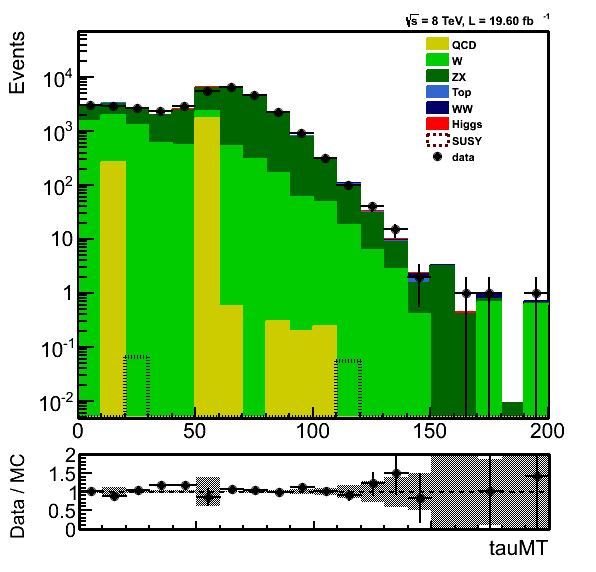
\includegraphics[width=0.45\textwidth,keepaspectratio=true]{ZValidation/tauMT_ZValidation.png}
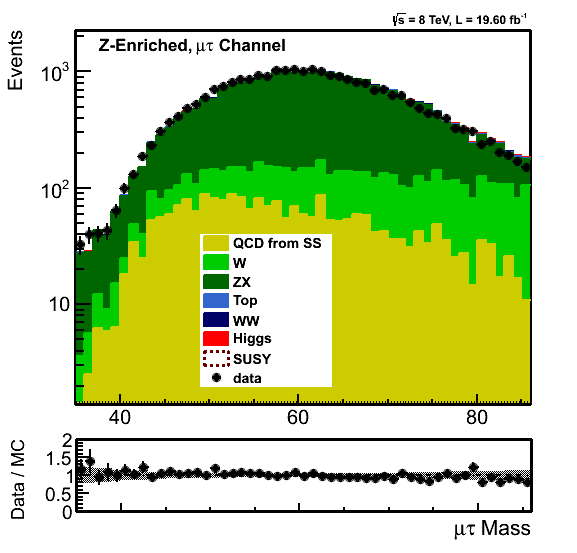
\includegraphics[width=0.45\textwidth,keepaspectratio=true]{ZValidation/InvMass_ZValidation.png}
\caption{left: \tauMT after all other selections to enrich \Z. right: data/MC comparison in the \Z peak.}
\label{fig:ZValidation}
\end{figure}
shows the \tauMT distribution after applying all other selections itemized above. Constraining the \tauMT between 40 and 100 \GeV can increase the \Z contamination from ~70\% to ~80\%. In figure \ref{fig:ZValidation} (right)
dilepton invariant mass is compared between data and MC. The QCD multijet in this plot is estimated from data. For this estimation, the same 
selection is applied as above except the charge of the \muTau which is same (SS) instead of opposite. This condition, enriches the selection 
by QCD multijets (~66\%). The non-QCD backgrounds read from MC are subtracted from data in this selection and the result is 
taken as QCD for OS selection.
It can be seen that data/MC have a good agreement in both shape and normalization under the \Z peak. {\bf FIXME} Evaluate a systematic to be assigned to Z MC.
